\documentclass{standalone}

\usepackage{tikz}

\newcommand{\interval}[3]{
\node at (#1,#3) {[};
\node at (#2,#3) {]};
\draw (#1,#3) -- (#2,#3);
}
\newcommand{\dottedinterval}[3]{
\node at (#1,#3) {[};
\node at (#2,#3) {]};
\draw[dotted] (#1,#3) -- (#2,#3);
}

\begin{document}

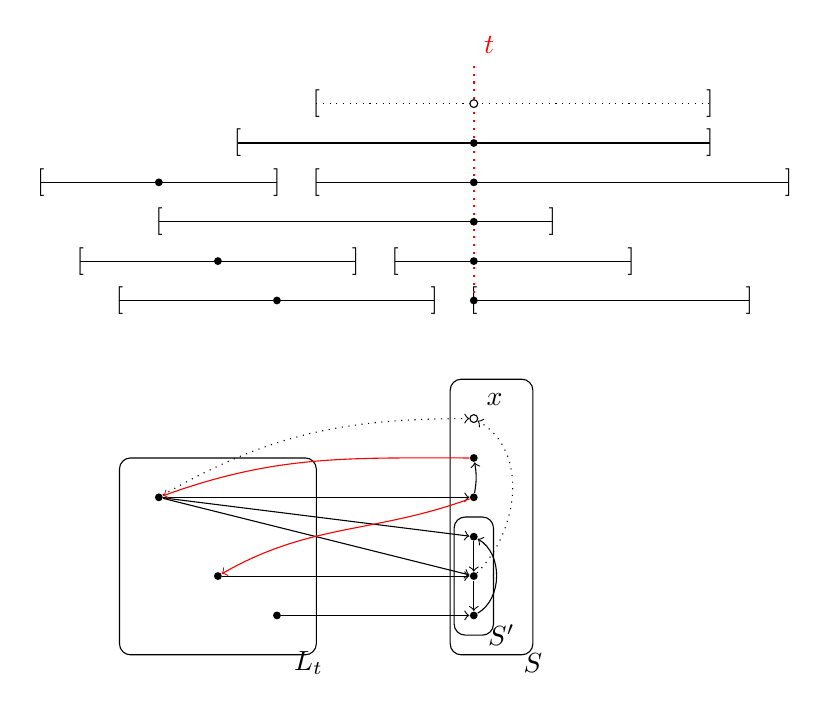
\begin{tikzpicture}
\interval{-3}{3}{3}
\interval{-2}{4}{2.5}
\interval{-4}{1}{2}
\interval{-1}{2}{1.5}
\interval{0}{3.5}{1}
\draw[red, thick, dotted] (0,1) -- node[at start, black, fill,circle, inner sep=1pt] {} node[at end,above right] {$t$} +(0,3);
\node[fill,circle,inner sep=1pt] at (0,1.5) {};
\node[fill,circle,inner sep=1pt] at (0,2) {};
\node[fill,circle,inner sep=1pt] at (0,2.5) {};
\node[fill,circle,inner sep=1pt] at (0,3) {};
\interval{-5}{-1.5}{1.5}
\node[fill,circle,inner sep=1pt] at (-3.25,1.5) {};
\interval{-5.5}{-2.5}{2.5}
\node[fill,circle,inner sep=1pt] at (-4,2.5) {};
\interval{-4.5}{-.5}{1}
\node[fill,circle,inner sep=1pt] at (-2.5,1) {};
\dottedinterval{-2}{3}{3.5}
\node[fill=white,draw=black,inner sep=1pt,circle] at (0,3.5) {};

\begin{scope}[shift={(0,-4)}]

\node[fill,circle,inner sep=1pt] (a) at (-2.5,1) {};
\node[fill,circle,inner sep=1pt] (b) at (0,1) {};
\node[fill,circle,inner sep=1pt] (c) at (-3.25,1.5) {};
\node[fill,circle,inner sep=1pt] (d) at (0,1.5) {};
\node[fill,circle,inner sep=1pt] (e) at (0,2) {};
\node[fill,circle,inner sep=1pt] (f) at (-4,2.5) {};
\node[fill,circle,inner sep=1pt] (g) at (0,2.5) {};
\node[fill,circle,inner sep=1pt] (h) at (0,3) {};
\node[fill=white,draw=black,inner sep=1pt,circle,label=above right:{$x$}] (i) at (0,3.5) {};

\draw[rounded corners] (-0.25,0.75) rectangle (0.25,2.25);
\node at (0.35,0.75) {$S'$};
\draw[rounded corners] (-0.3,0.5) rectangle (.75,4);
\node at (.75,0.4) {$S$};
\draw[rounded corners] (-4.5,0.5) rectangle (-2,3);
\node at (-2.1,0.4) {$L_t$};
\draw[->] (a) -- (b);
\draw[->] (c) -- (d);
\draw[->] (f) -- (g);
\draw[->] (f) -- (d);
\draw[->] (f) -- (e);
\draw[->] (e) -- (d);
\draw[->] (d) -- (b);
\draw[->] (b) to[in=-30,out=30] (e);
\draw[->,dotted] (f) to[out=30,in=180] (i);
\draw[->,dotted] (d) to[out=45,in=-30] (i);
\draw[->] (g) to[out=80,in=-80] (h);
\draw[->,red] (h) to[out=180,in=20] (f);
\draw[->,red] (g) to[out=200,in=30] (c);

\end{scope}

\end{tikzpicture}

\end{document}
